\chapter{Ocena eksperymentalna}
\section{Cel Badań}
Celem badań było sprawdzenie jak popularne algorytmy uczenia maszynowego radzą sobie z rozwiązaniem problemu 
klasyfikacji informacji jako prawdziwe lub nieprawdziwe. W celu sprawdzenia ich efektywności należało zbadać
takie cechy jak:
\begin{itemize}
    \item Czas fazy uczenia
    \item Czas fazy predykcji
    \item Procent poprawnych predykcji po nauczeniu modelu
\end{itemize}
W badaniach głównym sprawdzanym elementem było to jak zmiana długości NGramów na które podzielony
został tekst przed wektoryzacją wpływa na wyniki algorytmów i odnalezienie takiego rozmiaru, który
daje najlepsze wyniki. 

Do badania wybrano pięć popularnych algorytmów uczenia maszynowego są to: 
\begin{itemize}
    \item KNN - K najbliższych sąsiadów,
    \item SVM - maszyna wektorów nośnych,
    \item Naive Bayes,
    \item Random forest - las losowy,
    \item MLP - wielowarstwowy perceptron.
\end{itemize} 
\section{Warunki przeprowadzonego eksperymentu}
Badania zostały wykonane na komputerze stacjonarnym o następującej specyfikacji:
\begin{itemize}
    \item System operacyjny Windows 10 Pro w wersji 10.0.19041
    \item Procesor AMD Ryzen 5 3600
    \item Pamięć RAM 16 GB
\end{itemize}
Wszystkie badania były wykonywane w dokładnie takich samych warunkach aby można było 
je w prosty sposób porównywać. 

Dane badawcze to zbiór pod nazwą ``ISOT Fake News Dataset'' jest to przygotowany przez uczelnię w 
kanadzie ``Univerity of Victoria''. Zawiera on 12600 artykułów prawdziwych pochodzących ze strony
internetowej Reuters.com oraz 12600 artykułów nieprawdziwych zebranych z niewiarygodnych źródeł
oznaczonych przez organizację do sprawdzania faktów Politifact. Tematyka artykułów to głównie polityka i wiadomości 
ze świata.  Teksty zawarte w zbiorze zostały wstępnie przygotowane jednak błędy znajdujące się w nieprawdziwych 
artykułach pozostały w tekście. Zbiór został pobrany w dniu 16.06.2020 z witryny znajdującej się pod adresem \url{https://www.uvic.ca/}.~\cite{ISOT}

Algorytmy KNN, Random forest oraz Naive Bayes zostały zbadane na rozmiarach NGramów od 1 do 10 natomiast
MLP i SVC od 1 do 5 z powodu dużej złożoności obliczeniowej przy większym rozmiarze. Podczas
dzielenia danych na treningowe i testowe został wykorzystany parametr random\_state gwarantuje on
że dane zostaną zawsze podzielone w dokładnie taki sam sposób.
\section{Wyniki}
Wyniki badań przedstawiono poniżej, każdy z algorytmów został zbadany pod 
kątem 3 cech. Efektywność została zmierzona funkcją \textit{``Score''} na 40\% danych ze zbioru.
\begin{table}[H]
    \centering
    \caption{Wyniki algorytmu KNN wektoryzacja metodą Bag of words}
    \resizebox{\textwidth}{!}{%
    \begin{tabular}{ | l | c | c | c | c | c | c | c | c | c | c |}
        \hline
        Rozmiar Ngramu & 1 & 2 & 3 & 4 & 5 & 6 & 7 & 8 & 9 & 10  \\ \hline
        Efektywność & 75.65\% & 84.36\% & 63.52\% & 48.93\% & 47.5\% & 47.24\% & 47.23\% & 47.41\% & 61.48\% & 53.81\%  \\ \hline
        Czas fazy uczenia & 0.003s & 0.022s & 0.059s & 0.099s & 0.102s & 0.121s & 0.126s & 0.129s & 0.122s & 0.129s  \\ \hline
        Czas fazy predykcji & 27.221s & 180.565s & 312.157s & 221.672s & 137.788s & 91.407s & 67.833s & 54.803s & 45.88s & 40.02s  \\ \hline
    \end{tabular}
    }
\end{table}

\begin{table}[H]
    \centering
    \caption{Wyniki algorytmu KNN wektoryzacja metodą TFIDF}
    \resizebox{\textwidth}{!}{%
    \begin{tabular}{ | l | c | c | c | c | c | c | c | c | c | c |}
        \hline
        Rozmiar Ngramu & 1 & 2 & 3 & 4 & 5 & 6 & 7 & 8 & 9 & 10  \\ \hline
        Efektywność & 78.13\% & 71.26\% & 60.09\% & 64.01\% & 47.7\% & 47.54\% & 53.89\% & 53.66\% & 53.64\% & 53.63\%   \\ \hline
        Czas fazy uczenia & 0.003s & 0.024s & 0.067s & 0.092s & 0.112s & 0.111s & 0.122s & 0.123s & 0.127s & 0.129s \\ \hline
        Czas fazy predykcji & 27.168s & 186.84s & 321.7s & 220.716s & 141.115s & 93.327s & 68.613s & 46.536s & 47.467s & 37.644s  \\ \hline
    \end{tabular}
    }
\end{table}

\begin{table}[H]
    \centering
    \caption{Wyniki algorytmu Random Forest wektoryzacja metodą Bag of words}
    \resizebox{\textwidth}{!}{%
    \begin{tabular}{ | l | c | c | c | c | c | c | c | c | c | c |}
        \hline
        Rozmiar Ngramu & 1 & 2 & 3 & 4 & 5 & 6 & 7 & 8 & 9 & 10 \\ \hline
        Efektywność & 84.15\% & 98.09\% & 99.59\% & 99.81\% & 99.64\% & 99.33\% & 99.05\% & 98.81\% & 98.59\% & 98.29\%  \\ \hline
        Czas fazy uczenia & 23.56s & 47.484s & 48.267s & 45.867s & 52.639s & 73.57s & 108.591s & 143.566s & 187.709s & 225.265s \\ \hline
        Czas fazy predykcji & 0.234s & 0.764s & 2.587s & 5.095s & 6.324s & 8.315s & 15.628s & 19.665s & 23.49s & 25.823s  \\ \hline
    \end{tabular}
    }
\end{table}

\begin{table}[H]
    \centering
    \caption{Wyniki algorytmu Random Forest wektoryzacja metodą TFIDF}
    \resizebox{\textwidth}{!}{%
    \begin{tabular}{ | l | c | c | c | c | c | c | c | c | c | c |}
        \hline
        Rozmiar Ngramu & 1 & 2 & 3 & 4 & 5 & 6 & 7 & 8 & 9 & 10 \\ \hline
        Efektywność & 83.43\% & 98.15\% & 99.54\% & 99.82\% & 99.55\% & 99.27\% & 99.0\% & 98.62\% & 98.68\% & 98.24\%  \\ \hline
        Czas fazy uczenia & 26.536s & 57.014s & 53.246s & 47.681s & 48.82s & 63.392s & 92.896s & 132.436s & 175.463s & 217.02s \\ \hline
        Czas fazy predykcji & 0.24s & 0.729s & 3.027s & 5.021s & 6.554s & 7.893s & 14.047s & 20.172s & 24.588s & 26.493s  \\ \hline
    \end{tabular}
    }
\end{table}

\begin{table}[H]
    \centering
    \caption{Wyniki algorytmu Naive Bayes wektoryzacja metodą Bag of words}
    \resizebox{\textwidth}{!}{%
    \begin{tabular}{ | l | c | c | c | c | c | c | c | c | c | c |}
        \hline
        Rozmiar Ngramu & 1 & 2 & 3 & 4 & 5 & 6 & 7 & 8 & 9 & 10 \\ \hline
        Efektywność & 69.53\% & 78.91\% & 83.96\% & 92.19\% & 94.92\% & 96.12\% & 96.54\% & 96.67\% & 96.5\% & 96.29\%  \\ \hline
        Czas fazy uczenia & 0.005s & 0.031s & 0.102s & 0.147s & 0.201s & 0.377s & 0.551s & 0.692s & 0.837s & 1.027s \\ \hline
        Czas fazy predykcji & 0.003s & 0.016s & 0.047s & 0.072s & 0.095s & 0.182s & 0.299s & 0.362s & 0.382s & 0.41s  \\ \hline
    \end{tabular}
    }
\end{table}

\begin{table}[H]
    \centering
    \caption{Wyniki algorytmu Naive Bayes wektoryzacja metodą TFIDF}
    \resizebox{\textwidth}{!}{%
    \begin{tabular}{ | l | c | c | c | c | c | c | c | c | c | c |}
        \hline
        Rozmiar Ngramu & 1 & 2 & 3 & 4 & 5 & 6 & 7 & 8 & 9 & 10 \\ \hline
        Efektywność & 75.19\% & 81.98\% & 85.54\% & 92.43\% & 94.78\% & 96.11\% & 96.58\% & 96.71\% & 96.56\% & 96.38\%  \\ \hline
        Czas fazy uczenia & 0.005s & 0.033s & 0.105s & 0.159s & 0.193s & 0.293s & 0.504s & 0.675s & 0.853s & 1.02s \\ \hline
        Czas fazy predykcji & 0.002s & 0.017s & 0.05s & 0.077s & 0.09s & 0.145s & 0.319s & 0.343s & 0.406s & 0.407s  \\ \hline
    \end{tabular}
    }
\end{table}

\begin{table}[H]
    \centering
    \caption{Wyniki algorytmu SVC wektoryzacja metodą Bag of words}
    \begin{tabular}{ | l | c | c | c | c | c |}
        \hline
        Rozmiar Ngramu & 1 & 2 & 3 & 4 & 5 \\ \hline
        Efektywność & 81.36\% & 96.1\% & 97.75\% & 98.45\% & 98.34\%   \\ \hline
        Czas fazy uczenia & 14.175s & 319.6s & 2779.462s & 7282.055s & 10144.174s  \\ \hline
        Czas fazy predykcji & 8.18s & 127.618s & 716.666s & 1502.585s & 2534.03s  \\ \hline
    \end{tabular}
\end{table}

\begin{table}[H]
    \centering
    \caption{Wyniki algorytmu SVC wektoryzacja metodą TFIDF}
    \begin{tabular}{ | l | c | c | c | c | c |}
        \hline
        Rozmiar Ngramu & 1 & 2 & 3 & 4 & 5   \\ \hline
        Efektywność & 79.47\% & 96.61\% & 97.95\% & 98.65\% & 98.66\% \\ \hline
        Czas fazy uczenia & 14.046s & 220.009s & 3068.672s & 8322.766s & 10384.898s \\ \hline
        Czas fazy predykcji & 8.008s & 106.538s & 751.689s & 1594.27s & 2286.608s  \\ \hline
    \end{tabular}
\end{table}

\begin{table}[H]
    \centering
    \caption{Wyniki algorytmu MLP wektoryzacja metodą Bag of words}
    \begin{tabular}{ | l | c | c | c | c | c |}
        \hline
        Rozmiar Ngramu & 1 & 2 & 3 & 4 & 5  \\ \hline
        Efektywność & 81.68\% & 97.16\% & 98.6\% & 97.79\% & 98.37\%   \\ \hline
        Czas fazy uczenia & 32.655s & 22.982s & 115.108s & 544.161s & 2038.845s  \\ \hline
        Czas fazy predykcji & 0.039s & 0.11s & 0.373s & 1.085s & 2.444s  \\ \hline
    \end{tabular}
\end{table}

\begin{table}[H]
    \centering
    \caption{Wyniki algorytmu MLP wektoryzacja metodą TFIDF}
    \begin{tabular}{ | l | c | c | c | c | c |}
        \hline
        Rozmiar Ngramu & 1 & 2 & 3 & 4 & 5   \\ \hline
        Efektywność & 79.8\% & 97.43\% & 98.6\% & 98.69\% & 98.09\%   \\ \hline
        Czas fazy uczenia & 16.176s & 22.159s & 111.424s & 520.082s & 1926.648s  \\ \hline
        Czas fazy predykcji & 0.034s & 0.113s & 0.38s & 0.911s & 2.133s  \\ \hline
    \end{tabular}
\end{table}
\section{Analiza wyników wraz z oceną statystyczną}

Wyniki przeanalizowano pod kątem trzech badanych cech:

\begin{itemize}
    \item \textbf{Efektywność}
    
    \item \textbf{Czasy fazy uczenia}
    
    \item \textbf{Czasy fazy predykcji}
    
\end{itemize}
\begin{figure}[h!]
    \centering
    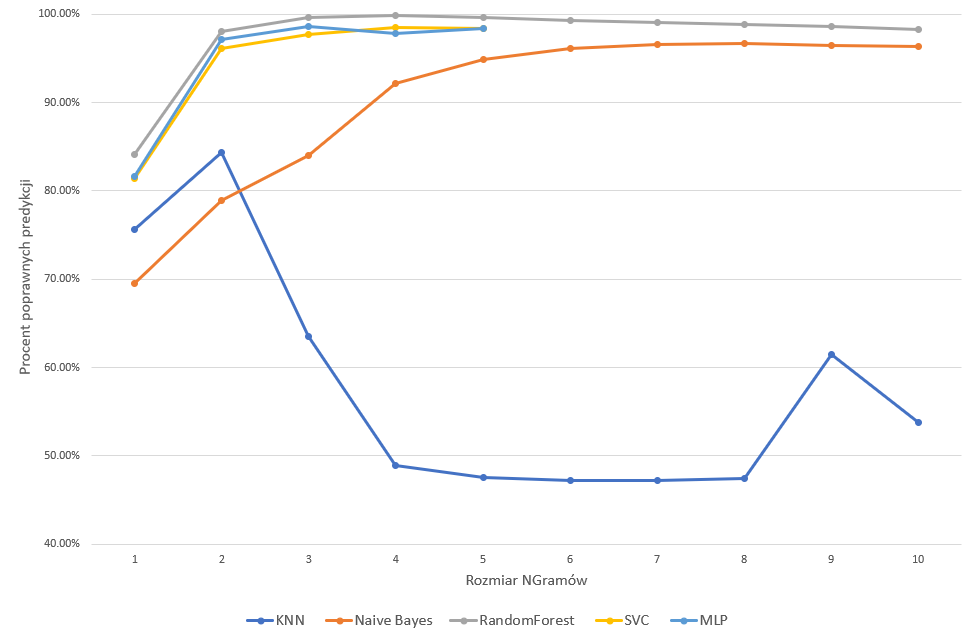
\includegraphics[width=0.9\textwidth]{./Img/BOWAcc.png}
    \caption{Efektywność algorytmów wektoryzacja metodą Bag of words}
\end{figure}

\begin{figure}[h!]
    \centering
    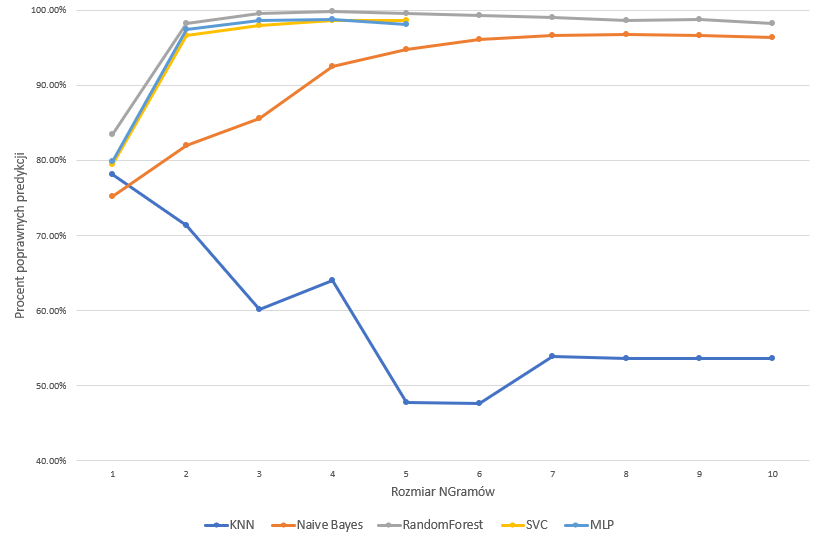
\includegraphics[width=0.9\textwidth]{./Img/TFIDFAcc.png}
    \caption{Efektywność algorytmów wektoryzacja metodą TFIDF}
\end{figure}

\begin{figure}[h!]
    \centering
    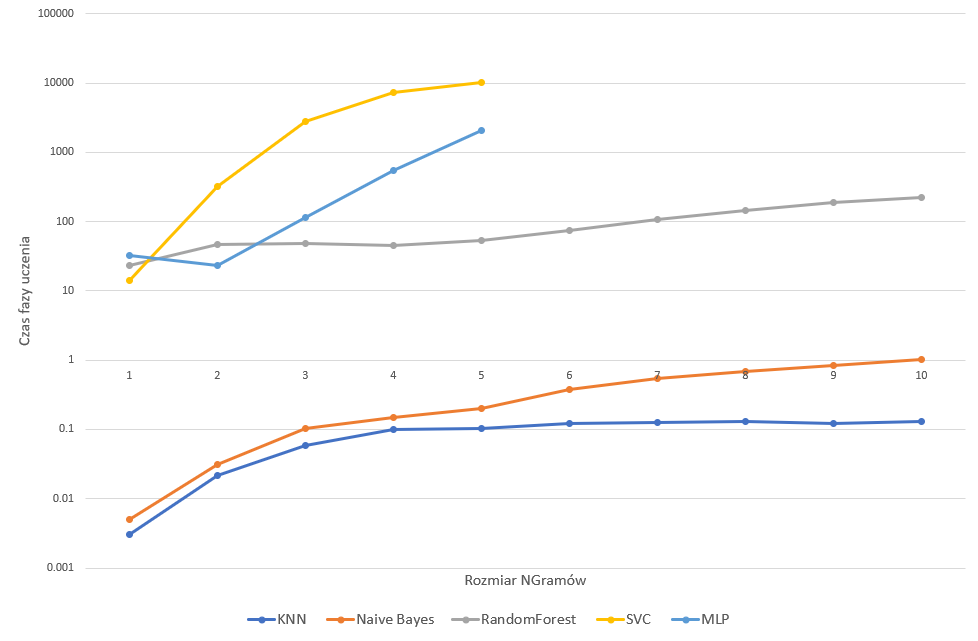
\includegraphics[width=0.9\textwidth]{./Img/BOWLearn.png}
    \caption{Czasy uczenia algorytmów wektoryzacja metodą Bag of words}
\end{figure}

\begin{figure}[h!]
    \centering
    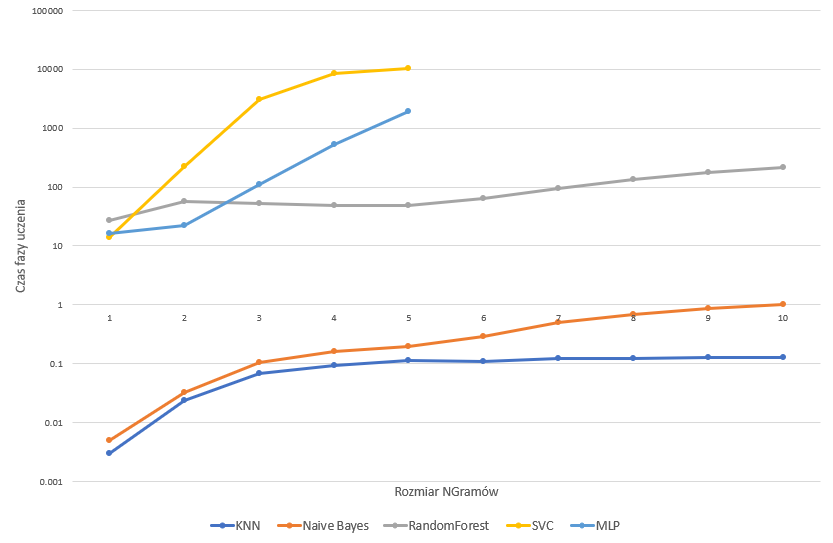
\includegraphics[width=0.9\textwidth]{./Img/TFIDFLearn.png}
    \caption{Czasy uczenia algorytmów wektoryzacja metodą TFIDF}
\end{figure}

\begin{figure}[h!]
    \centering
    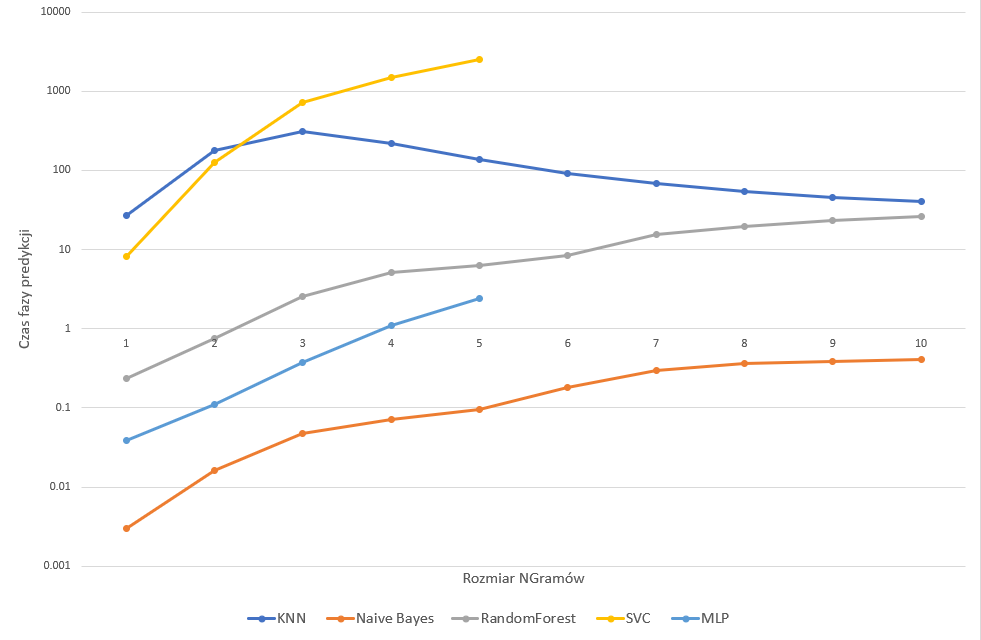
\includegraphics[width=0.9\textwidth]{./Img/BOWPredict.png}
    \caption{Czasy predykcji algorytmów wektoryzacja metodą Bag of words}
\end{figure}

\begin{figure}[h!]
    \centering
    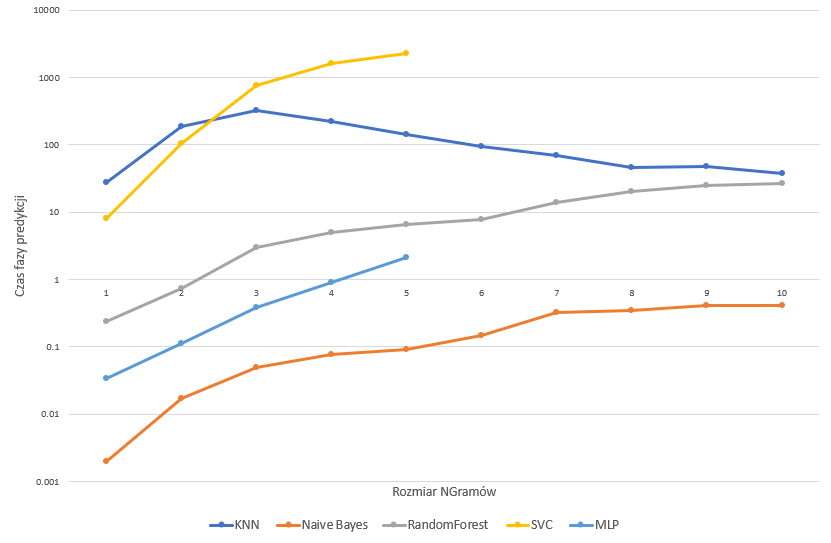
\includegraphics[width=0.9\textwidth]{./Img/TFIDFPredict.png}
    \caption{Czasy predykcji algorytmów wektoryzacja metodą TFIDF}
\end{figure}

\section{Wnioski z badań}
Przeprowadzone badania pozwoliły na odnalezienie odpowiedzi na pytanie 
będace celem niniejszej pracy.
